\chapter{Machine Learning}
\label{ch:machine_learning}
F: Was ist maschinelles lernen? welchen Zweck hat es?

Maschinelles Lernen (ML) ist \enquote{ein Forschungsfeld in der Schnittmenge von Statistik, künstlicher Intelligenz und Informatik}~\cite[S.~1]{Muller.2017}. Heute wird ML in vielen kommerziellen Bereichen genutzt; ebenso wie in der datengetriebenen Forschung. Die steigende Komplexität von Problemen hat dazu geführt, dass die individuelle Anfertigung von Programmen zur Lösung einer Problemstellung, häufig nicht mehr praktikabel ist. So muss ein ein Programm bereits für eine kleine Änderung der Problemstellung aufwendig überarbeitet werden oder die Aufgabe an sich übersteigt die Fähigkeit eines Experten, das Problem in seiner vollständigen Komplexität zu erfassen. Müller~\cite{Muller.2017} nennt in diesem Zusammenhang die Entwicklung von Gesichtserkennungssoftware als Beispiel. Er betont, dass aufgrund der grundsätzlich verschiedenen \enquote{Wahrnehmung} von Bildern zwischen Menschen und Computern, es für den Menschen unmöglich ist allgemeingültige Regeln zum Erkennen von Gesichtern zu definieren, die eine Software einsetzten könnte. Während Menschen einen optischen Eindruck von der Welt erhalten, sind Computer bei der Interpretation von Bildern auf Farbwerte einzelner Pixel angewiesen; sprich eine konkrete Menge diskreten Zahlenwerte. Die Entwicklung maschineller Lernalgorithmen hat es jedoch möglich gemacht das Erstellen von Entscheidungsmodellen weitgehend zu automatisieren.  

F: welche Unterkategorien gibt es beim machine learning?

Man unterscheidet beim maschinellen Lernen zwischen \textit{überwachten} und \textit{unüberwachten} Lernen. Beim überwachten Lernen werden dem Algorithmus Datenpunkte mit zugehörigem Zielwert übergeben. Im der Algorithmus verallgemeinernde Kriterien bestimmt an denen sich die Datenpunkte dem richtigen Zielwert zuordnen lassen, entsteht ein Model mit dem eine Zuordnung von zuvor unbekannten Datenpunkten getroffen werden kann. Der Zielwert kann dabei ein diskreter Wert (Klassifikation) oder eine kontinuierliche Variable (Regression) sein. Ein Beispiel für eine Klassifikationaufgabe eines überwachten Lernalgorithmus ist die Unterscheidung zwischen normalen Emails und Spam-Emails \cite[S.~2]{Muller.2017}.

Beim unüberwachten Lernen stehen für einen Datensatz keine Informationen über die Zielwerten zur Verfügung. Ziel dieses Ansatzes ist es Cluster in einem gegebenen Datensatz zu finden, um daraus weitere Schlüsse ziehen zu können.

F: Was hat ML mit PdM zutun?

Im Zuge der Digitalisierung von Produktionsprozessen stehen zunehmend größere Datenmengen zur Verfügung. Aus dieser Entwicklung folgt, dass Herausforderungen der Prozessoptimierung vom Datamining- und Machine Learning-Ansätzen profitieren können.~\cite[S.~35]{Schafer.25.09.201927.09.2019}

Die Einführung einer PdM-Anwendung anstelle einer anderen Instandhaltungsstrategie stellt einen Optimierungsprozess dar. Sowohl zur Klärung der Frage, ob die PdM-Anwendung eine Verbesserung darstellt, und für den Gebrauch der Anwendung müssen Modelle entwickelt werden, die die Verarbeitung der Anwendungsdaten ermöglichen. Maschinelle Lernalgorithmen sind dafür nützliche Tools, weil sie diese Prozesse vereinfachen (s.o.).
%===============================================================================
\section{Machine Learning Algorithmen mit Entscheidungsbäumen}
\label{sec:algorithmen_mit_entscheidungsbaum}
Entscheidungsbäume sind Entscheidungsstrukturen die auf der Teilung eines Datensatzes im mehreren Schritten beruhen. \cref{fig:entscheidungsbaum_schema} zeigt den prinzipiellen Aufbau eines Entscheidungsbaums.

\begin{wrapfigure}{r}{0.5\textwidth}
	\centering
	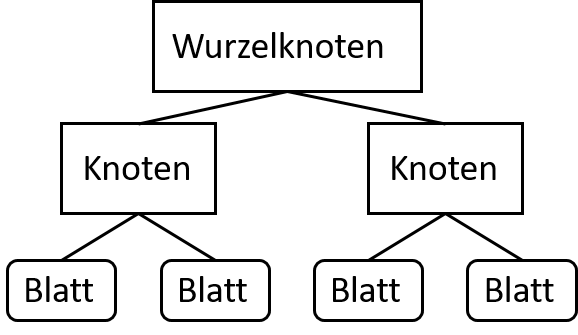
\includegraphics[width=0.48\textwidth]{entscheidungsbaum_aufbau.png}
	\caption{Schematische Darstellung eines Entscheidungsbaums}
	\label{fig:entscheidungsbaum_schema}
\end{wrapfigure}

Ein Datenpunkt wird durch einen Entscheidungsbaum einer Kategorie oder einem Wert zugeordnet. Zunächst wird anhand eines Merkmals eine Entscheidung im Wurzelknoten des Baums getroffen. Je nach Ergebnis wandert der Datenpunkt in einen der darunter liegenden Knoten. Hier wird nun ein anderes Merkmal beurteilt und der Datenpunkt entsprechend dem nächsten Knoten oder -- im letzten Schritt -- einem Blatt zugeordnet. Den Blättern sind die Kategorien oder Werte zugeordnet, welche mit jedem Datenpunkt assoziiert wird, welcher sich in dem Blatt befindet. 

Um das Entscheidungskriterium für jeden Knoten zu bestimmen, werden sämtliche möglichen Merkmale überprüft und der Wert bestimmt der den vorhandenen Datensatz am besten den richtigen Zielwerten zuordnen kann. Dies wird für alle Teilungen durch die Knoten wiederholt.~\cite{Muller.2017}

Ohne Beschränkungen würde ein Entscheidungsbaum solange weiter aufgebaut werden bis jedes Blatt nur einen einzelnen Datenpunkt enthält. Ein derart aufgebauter Entscheidungsbaum ist in der Regel ungeeignet, um damit zutreffende Zielwerte für neue Datenpunkte bestimmen zu können. Das Model orientiert sich zu stark an den Merkmalswerten aus dem Trainingsdatensatz und ist daher nicht in der Lage gute verallgemeinernde Entscheidungskriterien zu finden. Man spricht in diesem Zusammenhang von \textit{Overfitting}. Um Overfitting entgegen zu wirken kann beispielsweise die minimale Anzahl der Datenpunkte in einem Blatt limitiert werden oder die Tiefe des Baums und damit die Anzahl der Knoten begrenzt werden.

Es gibt verschiedenen Arten von ML-Modellen, die auf Entscheidungsbäumen basieren. Sie unterscheiden sich sowohl in der Strategie zum Aufbau der Bäume; der Anzahl der Bäume; als auch der Ermittlung des Gesamtergebnisses für einen Datenpunkt. 

Im weiteren Verlauf dieser Arbeit werden drei verschiedene maschinelle Lernalgorithmen angewendet, die auf Entscheidungsbäumen basieren. In den folgenden Abschnitten werden wichtige Eigenschaften dieser Modeltypen beleuchtet. Alle drei Modeltypen sind für die Programmiersprache \textit{Python} in dem Packet \textit{scikit-learn} implementiert.
%===============================================================================
\subsection{Einfache Entscheidungsbäume}
\label{sec:einfache_entscheidungsbaeume}
F: was ist das?

Der einfachste Modeltyp, der auf Entscheidungsbäumen beruht, ist ein einzelner Entscheidungsbaum. Wie in \cref{sec:algorithmen_mit_entscheidungsbaum} beschrieben, entspricht die Beurteilung eines Datenpunktes der Kategorie des Blatts, das den Datenpunkt beinhaltet.

Ein einzelner Entscheidungsbaum lässt sich praktikabel visualisieren; vorausgesetzt seine Knotenanzahl ist überschaubar. Das Verfahren nach dem der Baum Entscheidungen triff, kann so durch Sachverständige nachvollzogen und beurteilt werden. Dies ist der entscheidende Vorteil gegenüber anderen Modelarten, wie dem Random Forest oder den Gradient Boosted Trees.

Nachteil von Entscheidungsbäumen ist das sie zu Overfitting neigen~\cite[S.~80]{Muller.2017}. Selbst durch die Verwendung von \textit{Präpruning}-Parametern -- wie einer maximalen Baumtiefe -- lässt sich Overfitting nicht gänzlich verhindern~\cite[S.~80]{Muller.2017}. Dennoch ist es laut Müller~\cite[S.~79]{Muller.2017} in der Regel ausreichend nur einen Parameter für Präpruning zu setzten.
%===============================================================================
\subsection{Random Forests}
\label{sec:random_forest}
F: Was ist das?

\textit{Random Forests} gehören zu den \textit{Ensembles} von Entscheidungsbäumen. Ensembles kombinieren mehrere Modelle miteinander um ein komplexeres Model zu generieren. Im Fall des Random Forest wird eine Vielzahl von Entscheidungsbäumen trainiert. Als Entscheidung eines Random Forest wird der gemittelte Wert aller Bäume gewählt. Die einzelnen Bäume können sich in all ihren Eigenschaften von einander unterscheiden. Das beinhaltet neben der Größe auch die Wahl der verwendeten Merkmale. Jeder Baum wird also unabhängig von den anderen konstruiert. Mit einer großen Anzahl von Bäume, die alle unterschiedliche Entscheidungskriterien verwenden und dennoch passable Ergebnisse liefern, können Random Forests Overfitting weitgehend reduzieren \cite{Muller.2017}.

F: was sind vorteile - und nachteile?

Durch die große Anzahl an Bäumen sind Random Forests wesentlich komplexer als einfache Entscheidungsbäume. Bei geeigneten Parametereinstellungen lassen sich so bessere Ergebnisse erzielen als bei einfachen Entscheidungsbäumen. Da zum Aufbau eines Random Forest aber viele Entscheidungsbäume erstellt werden müssen ist der Rechenaufwand relativ hoch~\cite[S.~84]{Muller.2017}. Laut Müller~\cite[S.~85]{Muller.2017} sind Random Forests außerdem nicht für dünn besetzte Datensätze geeignet.

Nach Müller~\cite[S.~85]{Muller.2017} sind die wichtigsten Parameter eines Random Forest die Anzahl der Klassifikatoren, die Anzahl maximal zu verwendender Merkmale und ein Parameter zum Prä-Pruning.
%===============================================================================
\subsection{Gradient Boosted Trees}
\label{sec:gradient_boosted_trees}
F: was ist das?

Gradient Boosted Trees (GBT) ist, wie der Random Forest, eine Ensembles-Methode. GBT beziehen im Gegensatz zum Random Forest die Ergebnisse der einzelnen Bäume nicht parallel, sondern nacheinander in die Gesamtbewertung mit ein. GBT versucht den Fehler eines Baums im nachfolgenden bestmöglich zu beheben. Dies setzt sich durch die gesamte Reihe an Bäumen fort.

F: was sind vorteile - und nachteile?

Laut Müller~\cite{Muller.2017} sind die wichtigsten Parameter von GBT die Lernrate und die Anzahl der Bäume. Demnach gewähre eine höhere Lernrate dem GBT die Möglichkeit mit jedem Baum die Fehler des Vorherigen stärker zu korrigieren. Je größer die Baumanzahl ist desto häufiger kann der Korrekturvorgang wiederholt werden, um das Ergebnis zu verbessern. Beide Parameter beeinflussen die Komplexität des Models. Müller~\cite{Muller.2017} weißt auch darauf hin, dass eine höhere Baumanzahl nicht zwangsläufig zu einer Verbesserung des Models führt, wie beim Random Forest. GBT neige bei großen Anzahlen an Bäumen zu Overfitting. Für den Fall, dass Overfitting in Zusammenhang mit einer hohen Baumanzahl vermutet wird, sollte daher die Anzahl reduziert werden, bis vertrauenswürdigere Ergebnisse beobachtet werden können.

Als relevanteste Vorteilen von GBT nennt Müller~\cite{Muller.2017}, dass derartige Modelle in vielen Fällen hohe Genauigkeiten im Vergleich zu anderen Modeltypen liefern; vorausgesetzt die Parameter sind geeignet eingestellt.
%===============================================================================